%% ----------------------------------------------------------------------------
%%  §11.8  Convergenza assoluta
%% ----------------------------------------------------------------------------
\section{Convergenza assoluta}
\label{sec:convergenza-assoluta}

Per una serie a termini di segno qualsiasi, il primo passo è spesso studiare la serie
dei valori assoluti, che è a termini non negativi e alla quale si applicano tutti i
criteri del \S\ref{sec:criteri-convergenza}.

\begin{definizione}[Convergenza assoluta]\label{def:convergenza-assoluta}
\index{serie!assolutamente convergente}
La serie $\sum a_{k}$ si dice \emph{assolutamente convergente} se è convergente la serie dei
valori assoluti
\begin{equation}\label{eq:serie-valori-assoluti}
  \sum_{k=1}^{\infty}\abs{a_{k}}=\abs{a_{1}}+\abs{a_{2}}+\dots+\abs{a_{n}}+\cdots .
\end{equation}
\end{definizione}

Una serie convergente non è necessariamente assolutamente convergente: la serie armonica
alternata converge, ma la serie dei suoi valori assoluti è la serie armonica, che
diverge. Una serie convergente ma non assolutamente convergente si dice
\emph{semplicemente} (o \emph{condizionatamente}) convergente. Il viceversa, invece, vale.

\begin{teorema}[La convergenza assoluta implica la convergenza]
\label{teo:convergenza-assoluta}
Una serie assolutamente convergente è convergente, e
\begin{equation}\label{eq:disuguaglianza-serie}
  \Bigl|\sum_{k=1}^{\infty}a_{k}\Bigr|\le\sum_{k=1}^{\infty}\abs{a_{k}} .
\end{equation}
\end{teorema}

\needspace{9\baselineskip}
\begin{schema}
\Ipotesi{$\sum\abs{a_{k}}<+\infty$.}
\Tesi{$\sum a_{k}$ converge e $\abs{\sum a_{k}}\le\sum\abs{a_{k}}$.}
\end{schema}

\begin{strategia}
Non conosciamo la somma della serie, e quindi conviene un criterio che non la richieda:
quello di Cauchy. I blocchi di termini consecutivi della serie data sono, per la
disuguaglianza triangolare, più piccoli dei corrispondenti blocchi della serie dei valori
assoluti, che verificano la condizione di Cauchy perché questa serie converge. Daremo
anche una seconda dimostrazione, che riconduce il problema a serie a termini non
negativi.
\end{strategia}

\begin{dimostrazione}[Prima dimostrazione (con il criterio di Cauchy)]
Poiché $\sum\abs{a_{k}}$ converge, per il criterio di Cauchy (\cref{teo:cauchy-serie}), dato
$\epsilon>0$ esiste $\nu$ tale che $\sum_{k=n+1}^{n+p}\abs{a_{k}}<\epsilon$ per ogni $n>\nu$ e ogni $p\in\N$. Per gli
stessi indici, per la disuguaglianza triangolare,
\[
  \Bigl|\sum_{k=n+1}^{n+p}a_{k}\Bigr|\le\sum_{k=n+1}^{n+p}\abs{a_{k}}<\epsilon ,
\]
e quindi, ancora per il criterio di Cauchy, la serie $\sum a_{k}$ converge. Infine, per
ogni $n$, $\abs{\sum_{k=1}^{n}a_{k}}\le\sum_{k=1}^{n}\abs{a_{k}}$; passando al limite (il valore assoluto è
continuo e le disuguaglianze larghe si conservano) si ottiene la
\eqref{eq:disuguaglianza-serie}.
\end{dimostrazione}

\begin{dimostrazione}[Seconda dimostrazione (con il confronto)]
Per ogni $k$ si ha $0\le a_{k}+\abs{a_{k}}\le2\abs{a_{k}}$. La serie di termine generale $2\abs{a_{k}}$
converge, e per il criterio del confronto converge anche la serie a termini non negativi
$\sum(a_{k}+\abs{a_{k}})$. Allora, per la linearità (\cref{prop:linearita-serie}), converge
anche la serie
\[
  \sum_{k=1}^{\infty}a_{k}=\sum_{k=1}^{\infty}\bigl(a_{k}+\abs{a_{k}}\bigr)-\sum_{k=1}^{\infty}\abs{a_{k}} ,
\]
differenza di due serie convergenti. La \eqref{eq:disuguaglianza-serie} si dimostra come
nella prima dimostrazione.
\end{dimostrazione}

Applicando i criteri del \S\ref{sec:criteri-convergenza} alla serie dei valori assoluti si
ottengono criteri di convergenza per serie a termini di segno qualsiasi. Ad esempio, dai
criteri del rapporto e della radice:

\begin{corollario}\label{cor:rapporto-assoluto}
Sia $a_{n}\neq0$ e supponiamo che esista $\ell=\lim\frac{\abs{a_{n+1}}}{\abs{a_{n}}}$ oppure
$\ell=\lim\sqrt[n]{\abs{a_{n}}}$. Se $\ell<1$ la serie $\sum a_{k}$ converge assolutamente; se $\ell>1$ la
serie non converge.
\end{corollario}

\begin{schema}
\Ipotesi{$a_{n}\neq0$; \ $\frac{\abs{a_{n+1}}}{\abs{a_{n}}}\to\ell$ oppure $\sqrt[n]{\abs{a_{n}}}\to\ell$.}
\Tesi{$\ell<1\implica\sum a_{k}$ assolutamente convergente; \ $\ell>1\implica\sum a_{k}$ non converge.}
\end{schema}

\begin{strategia}
Si applicano i criteri del rapporto e della radice alla serie dei valori assoluti. Per
$\ell<1$ si conclude con il teorema appena dimostrato; per $\ell>1$ si riutilizza ciò che le
dimostrazioni di quei criteri hanno mostrato: il termine generale non tende a zero.
\end{strategia}

\begin{dimostrazione}
Se $\ell<1$, la serie $\sum\abs{a_{k}}$ converge per il \cref{teo:criterio-rapporto-serie} o per il
\cref{teo:criterio-radice}, e si applica il \cref{teo:convergenza-assoluta}. Se $\ell>1$, nelle
dimostrazioni di quei criteri abbiamo visto che $\abs{a_{n}}$ non tende a zero; allora neppure
$a_{n}$ tende a zero, e la serie non converge per il \cref{teo:condizione-necessaria}.
\end{dimostrazione}

\begin{esempio}\label{es:assoluta}
\begin{enumerate}[label=(\alph*)]
  \item $\sum\frac{\sen k}{k^{2}}$ converge assolutamente, perché $\frac{\abs{\sen k}}{k^{2}}\le\frac1{k^{2}}$. I segni dei
  suoi termini non seguono alcuno schema regolare: il criterio di Leibniz non sarebbe
  applicabile.
  \item La serie esponenziale $\sum\frac{x^{k}}{k!}$ converge assolutamente per \emph{ogni}
  $x\in\R$: il rapporto dei valori assoluti è $\frac{\abs x}{n+1}\to0$.
  \item $\sum\frac{(-1)^{k}}{\sqrt k}$ converge per il criterio di Leibniz, ma non assolutamente,
  perché $\sum\frac1{\sqrt k}$ diverge ($p=\frac12$).
\end{enumerate}
\end{esempio}

\subsection{Riordinare una serie}

In una somma finita l'ordine degli addendi è irrilevante. Per le serie la questione è
delicata, perché la somma è un limite, e il limite dipende dall'ordine in cui si
presentano le somme parziali. Un \emph{riordinamento} della serie $\sum a_{k}$ è una serie
$\sum a_{\sigma(k)}$, dove $\sigma:\N\to\N$ è una funzione biunivoca: gli stessi termini, ciascuno
preso una e una sola volta, in un ordine diverso.

\begin{teorema}[di Dirichlet]\label{teo:dirichlet-riordinamento}
\index{teorema!di Dirichlet sui riordinamenti}
Se la serie $\sum a_{k}$ è assolutamente convergente, ogni suo riordinamento è
assolutamente convergente e ha la stessa somma.
\end{teorema}

\begin{schema}
\Ipotesi{$\sum\abs{a_{k}}<+\infty$; \ $\sigma:\N\to\N$ biunivoca.}
\Tesi{$\sum a_{\sigma(k)}$ converge assolutamente e $\sum_{k=1}^{\infty}a_{\sigma(k)}=\sum_{k=1}^{\infty}a_{k}$.}
\end{schema}

\begin{strategia}
Per le serie a termini non negativi la somma è l'estremo superiore delle somme parziali,
e ogni somma parziale della serie riordinata è maggiorata da una somma parziale della
serie data (basta prendere abbastanza termini da includere tutti quelli usati): dunque la
somma riordinata non supera quella originale, e per simmetria vale anche il viceversa.
Il caso generale si riconduce a questo scrivendo ogni termine come differenza della sua
parte positiva e della sua parte negativa.
\end{strategia}

\begin{dimostrazione}
\emph{Primo passo: $a_{k}\ge0$.} Sia $s=\sum a_{k}$ e sia $t_{n}=\sum_{k=1}^{n}a_{\sigma(k)}$. Posto
$N=\max\{\sigma(1),\dots,\sigma(n)\}$, gli indici $\sigma(1),\dots,\sigma(n)$ sono distinti e compresi tra $1$ e $N$,
e poiché i termini sono non negativi $t_{n}\le\sum_{j=1}^{N}a_{j}\le s$. Dunque la serie riordinata, a
termini non negativi, converge (\cref{teo:serie-positive}) e la sua somma $t$ verifica
$t\le s$. Ma la serie data è a sua volta un riordinamento di quella riordinata (mediante
la funzione inversa $\sigma^{-1}$), e lo stesso ragionamento dà $s\le t$. Quindi $t=s$.

\emph{Secondo passo: caso generale.} Poniamo $a_{k}^{+}=\max\{a_{k},0\}$ e $a_{k}^{-}=\max\{-a_{k},0\}$, in modo
che $a_{k}=a_{k}^{+}-a_{k}^{-}$ e $\abs{a_{k}}=a_{k}^{+}+a_{k}^{-}$. Poiché $0\le a_{k}^{\pm}\le\abs{a_{k}}$, le serie $\sum a_{k}^{+}$ e
$\sum a_{k}^{-}$ convergono per il confronto. Per il primo passo, applicato alle serie
$\sum\abs{a_{k}}$, $\sum a_{k}^{+}$ e $\sum a_{k}^{-}$, i loro riordinamenti convergono alle stesse somme; in
particolare $\sum a_{\sigma(k)}$ converge assolutamente e, per la linearità,
\[
  \sum_{k=1}^{\infty}a_{\sigma(k)}=\sum_{k=1}^{\infty}a_{\sigma(k)}^{+}-\sum_{k=1}^{\infty}a_{\sigma(k)}^{-}
  =\sum_{k=1}^{\infty}a_{k}^{+}-\sum_{k=1}^{\infty}a_{k}^{-}=\sum_{k=1}^{\infty}a_{k} . \qedhere
\]
\end{dimostrazione}

Per le serie semplicemente convergenti la situazione è opposta, e sorprendente.

\begin{esempio}[Un riordinamento della serie armonica alternata]\label{es:riordinamento}
Sia $L=\log2=1-\frac12+\frac13-\frac14+\cdots$. Moltiplicando per $\frac12$ (\cref{prop:linearita-serie})
e intercalando degli zeri, il che non cambia né il carattere né la somma
(\cref{oss:termini-nulli}),
\[
  \tfrac12L=0+\tfrac12+0-\tfrac14+0+\tfrac16+0-\tfrac18+\cdots .
\]
Sommando termine a termine con la serie di $L$, ancora per la linearità,
\[
  \tfrac32L=1+0+\tfrac13-\tfrac12+\tfrac15+0+\tfrac17-\tfrac14+\cdots ,
\]
e, togliendo gli zeri (ancora per l'\cref{oss:termini-nulli}),
\begin{equation}\label{eq:riordinamento}
  1+\frac13-\frac12+\frac15+\frac17-\frac14+\frac19+\frac1{11}-\frac16+\dots=\frac32\log2 .
\end{equation}
Il primo membro contiene esattamente i termini della serie armonica alternata, ciascuno
una volta, in un ordine diverso (due positivi e un negativo): è un suo riordinamento, ma
la somma è aumentata del $50\%$ (\cref{fig:riordinamento}).
\end{esempio}

Il fenomeno è del tutto generale, come dimostrò Riemann; ci limitiamo a enunciare il
risultato e a descrivere l'idea della dimostrazione.

\begin{teorema}[di Riemann, senza dimostrazione]\label{teo:riemann-riordinamento}
\index{teorema!di Riemann sui riordinamenti}
Se la serie $\sum a_{k}$ è semplicemente convergente, per ogni $L\in\overline\R$ esiste un suo
riordinamento che ha somma $L$; esistono inoltre riordinamenti indeterminati.
\end{teorema}

\begin{schema}
\Ipotesi{$\sum a_{k}$ convergente; \ $\sum\abs{a_{k}}=+\infty$; \ $L\in\overline\R$.}
\Tesi{esiste $\sigma:\N\to\N$ biunivoca con $\sum_{k=1}^{\infty}a_{\sigma(k)}=L$; \ esistono
riordinamenti indeterminati.}
\end{schema}

\begin{strategia}[Idea della dimostrazione]
Le serie $\sum a_{k}^{+}$ delle parti positive e $\sum a_{k}^{-}$ delle parti negative sono entrambe
divergenti (se una convergesse, convergerebbe anche l'altra, e quindi la serie dei valori
assoluti), mentre $a_{k}\to0$. Per ottenere la somma $L\in\R$ si prendono termini positivi
finché la somma parziale supera $L$, poi termini negativi finché scende sotto $L$, e così
via: le risorse non si esauriscono mai, perché ciascuna delle due serie diverge, e le
oscillazioni attorno a $L$ sono maggiorate dagli ultimi termini usati, che tendono a zero.
\end{strategia}

Il programma che segue mette in pratica questo algoritmo.

\begin{figure}[htb]
\centering
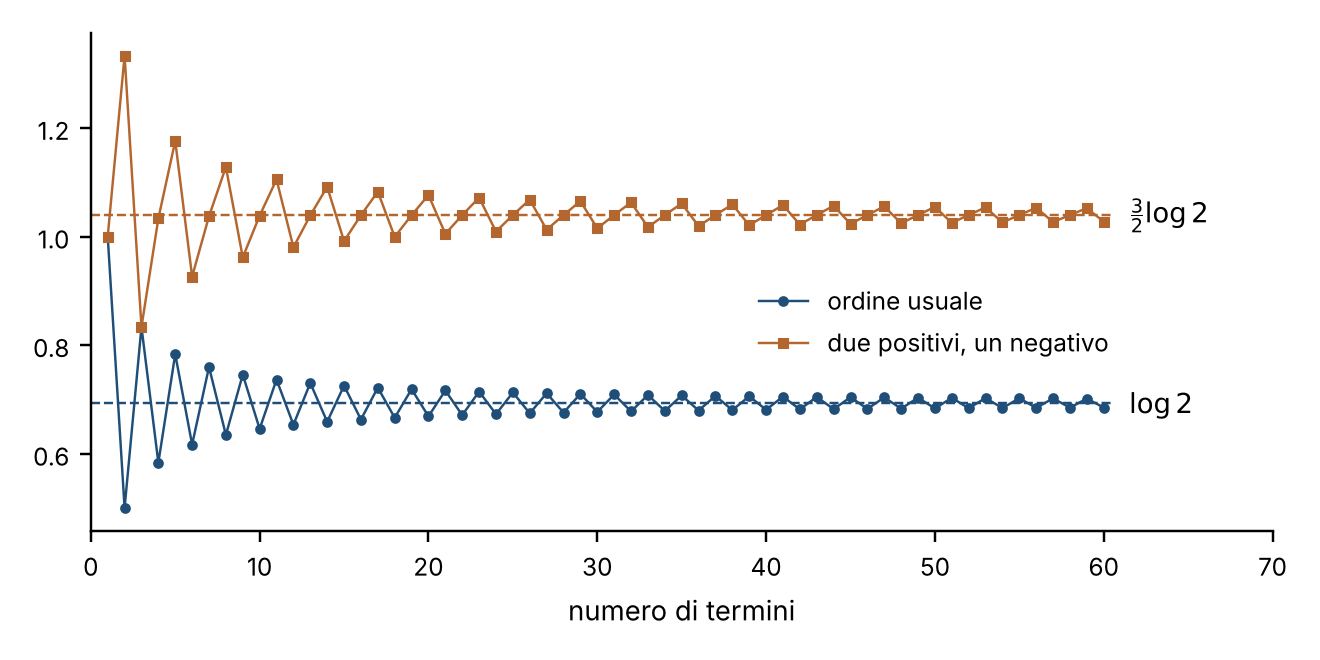
\includegraphics[width=\textwidth]{figure/riordinamento.png}
\caption{Somme parziali della serie armonica alternata nell'ordine usuale (blu), che
convergono a $\log2$, e del riordinamento \eqref{eq:riordinamento} con due termini positivi
e uno negativo (rame), che convergono a $\frac32\log2$. Gli stessi termini, sommati in un
ordine diverso, danno una somma diversa (\texttt{python/fig\_riordinamento.py}).}
\label{fig:riordinamento}
\end{figure}

\needspace{10\baselineskip}
\begin{python}[Riordinamenti della serie armonica alternata]
import math

def riordina(L, N):
    """Somma N termini di 1 - 1/2 + 1/3 - ... riordinati in modo
    che le somme parziali tendano a L (algoritmo di Riemann)."""
    s, p, q = 0.0, 1, 2          # prossimo dispari, prossimo pari
    for _ in range(N):
        if s <= L:
            s += 1 / p; p += 2   # termine positivo
        else:
            s -= 1 / q; q += 2   # termine negativo
    return s

s, p, q = 0.0, 1, 2              # due positivi e un negativo
for _ in range(100000):
    s += 1 / p + 1 / (p + 2) - 1 / q
    p, q = p + 4, q + 2
print(f"due +, un -:  {s:.6f}   (3/2) log 2 = {1.5*math.log(2):.6f}")
for L in (0.0, 1.0, math.pi):
    print(f"obiettivo L = {L:.6f}:  "
          f"somma = {riordina(L, 10**6):.6f}")
\end{python}
\begin{risultato}
due +, un -:  1.039718   (3/2) log 2 = 1.039721
obiettivo L = 0.000000:  somma = -0.000000
obiettivo L = 1.000000:  somma = 1.000000
obiettivo L = 3.141593:  somma = 3.141585
\end{risultato}

\begin{osservazione}
Il teorema di Dirichlet ha una conseguenza pratica: i termini di una serie
assolutamente convergente si possono raggruppare e riordinare nel modo più conveniente
senza alterare la somma, ad esempio sommando separatamente i termini positivi e quelli
negativi, o calcolando a parte certi blocchi di termini di cui si conosce la somma. Per
una serie semplicemente convergente, invece, l'ordine dei termini fa parte della
definizione stessa della serie. (Un'altra cosa è l'ordine in cui il calcolatore esegue
le addizioni di una somma parziale, che è una somma \emph{finita}: lì sommare dal termine
più piccolo al più grande riduce gli errori di arrotondamento, senza bisogno di alcun
teorema.)
\end{osservazione}

\begin{notastorica}[Cauchy, Dirichlet, Riemann]
Per tutto il Settecento le serie furono usate con grande disinvoltura, e talvolta con
risultati contraddittori. Fu Augustin-Louis Cauchy, nel \emph{Cours d'analyse} del 1821, a
fondarne la teoria sulla definizione di somma come limite delle somme parziali, con il
criterio che porta il suo nome (anticipato da Bernard Bolzano nel 1817), il criterio
della radice e quello di condensazione; quello del rapporto era già stato usato da d'Alembert. Nel 1837 Peter
Gustav Lejeune Dirichlet osservò che il valore di una serie semplicemente convergente
dipende dall'ordine dei termini e dimostrò che ciò non accade per le serie
assolutamente convergenti. Bernhard Riemann dimostrò il teorema che porta il suo nome nella
dissertazione di abilitazione sulle serie trigonometriche (1854), pubblicata postuma nel
1867.
\end{notastorica}
